\documentclass[../main.tex]{subfiles}

\begin{document}
In this chapter, we focusing on solving problems that carried on or the solution is related using non-linear data structures that are not array/string, such as linked list, heap, queue, and stack. 
%%%%%%%%%%%%%Linked List%%%%%%%%%%%%%%%%%%%%%%%
\section{Linked List}
Problems with linked list can be basic operations to add or remove node, or merge two different linked list. 
\paragraph{Circular Linked List} For the circular linked list, when we are traversing the list, the most important thing is to know how to set up the end condition for the while loop. 
\begin{examples}[resume]
\item \textbf{708. Insert into a Cyclic Sorted List (medium)} Given a node from a cyclic linked list which is sorted in ascending order, write a function to insert a value into the list such that it remains a cyclic sorted list. The given node can be a reference to any single node in the list, and may not be necessarily the smallest value in the cyclic list. For example,
\begin{figure}[h!]
    \centering
    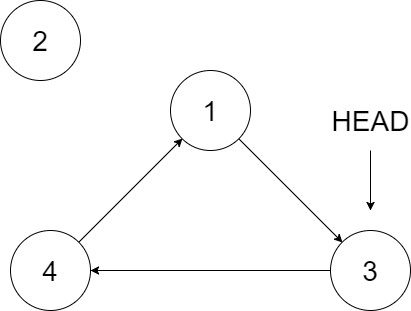
\includegraphics[width=0.5\columnwidth]{fig/insertcyclicbefore.png}
    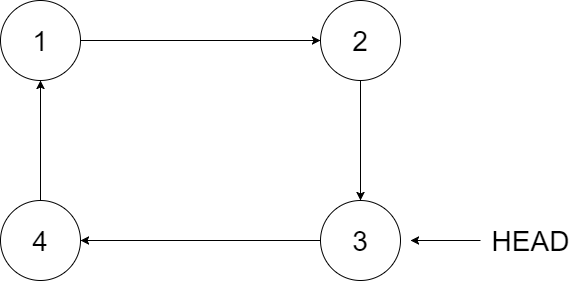
\includegraphics[width=0.5\columnwidth]{fig/insertcyclicafter.png}
    \caption{Example of insertion in circular list}
    \label{fig:circular list}
\end{figure}

\textbf{Analysis:} The maximum we traverse the list is one round. The potential positions we insert is related to the insert value. Suppose the linked list is in range of [s, e], s<=e.  Given the insert value as m:
\begin{enumerate}
    \item $m\in [s, e]$: we insert in the middle of the list. 
    \item $ m \geq e$ or $ m\leq s$: we insert at the end of the list, we need to detect the end as if the current node's value is larger than its successor's value. 
    \item After one loop, if we can not find a place, then we insert at the end. For example, 2->2->2 and insert 3 or 2->3->4->2 and insert 2. 
\end{enumerate}
\begin{lstlisting}[language=Python]
def insert(self, head, insertVal):
    if not head: # 0 node
        head = Node(insertVal,None)
        head.next = head
        return head         
    
    cur = head
    while cur.next != head:
        if cur.val <= insertVal <= cur.next.val: # insert
            break
        elif cur.val > cur.next.val: # end and start
            if insertVal >= cur.val or insertVal <= cur.next.val:
                break
            cur = cur.next
        else:
            cur = cur.next
    # insert
    node = Node(insertVal,None)
    node.next, cur.next = cur.next, node
    return head
\end{lstlisting}
\end{examples}
%%%%%%%%%%%%%queue and stack%%%%%%%%%%%%%%%%%%%%%%%
\section{Queue and Stack}
Because Queue and Stack is used to implement BFS and DFS search respectively, therefore, that type of implementation is covered in Chapter~\ref{graph_problem}.  The other problems include: Buffering problem with Queue(circular queue), 
%%%%%%%%%%%%%%%%%%Implementation%%%%%%%%%%%%%%%%%%%%%%%%%%
\subsection{Implementing Queue and Stack}
\begin{examples}[resume]
\item \textbf{622. Design Circular Queue (medium).} Design your implementation of the circular queue. The circular queue is a linear data structure in which the operations are performed based on FIFO (First In First Out) principle and the last position is connected back to the first position to make a circle. It is also called \textbf{"Ring Buffer"}.

Your implementation should support following operations:
\begin{itemize}
    \item MyCircularQueue(k): Constructor, set the size of the queue to be k.
    \item Front: Get the front item from the queue. If the queue is empty, return -1.
    \item Rear: Get the last item from the queue. If the queue is empty, return -1.
    \item enQueue(value): Insert an element into the circular queue. Return true if the operation is successful.
    \item deQueue(): Delete an element from the circular queue. Return true if the operation is successful.
    \item isEmpty(): Checks whether the circular queue is empty or not.
    \item isFull(): Checks whether the circular queue is full or not.
\end{itemize}

\textbf{Solution 1: Singly Linked List with Predefined Size.} This is a typical queue data structure and because it is a buffering, therefore, we need to limit its size. As shown in previous theory chapter of the book, queue can be implemented with singly linked list with two pointers, one at the head and the other at the rear. The additional controlling we need is to limit the size of the queue.
\begin{lstlisting}[language=Python]
class MyCircularQueue:
    class Node:
         def __init__(self, val):
                self.val = val
                self.next = None
    def __init__(self, k):
        self.size = k
        self.head = None
        self.tail = None
        self.cur_size = 0       

    def enQueue(self, value):
        if self.cur_size >= self.size:
            return False
        new_node = MyCircularQueue.Node(value)
        if self.cur_size == 0:
            self.tail = self.head = new_node
        else:
            self.tail.next = new_node
            new_node.next = self.head
            self.tail = new_node
        self.cur_size += 1
        return True        

    def deQueue(self):

        if self.cur_size == 0:
            return False
        # delete head node
        val = self.head.val
        if self.cur_size == 1:
            self.head = self.tail = None
        else:
            self.head = self.head.next
        self.cur_size -= 1
        return True    

    def Front(self):
        return self.head.val if self.head else -1

    def Rear(self):
        return self.tail.val if self.tail else -1

    def isEmpty(self):        
        return True if self.cur_size == 0 else False
    
    def isFull(self):
        return True if self.cur_size == self.size else False
\end{lstlisting}
\item \textbf{641. Design Circular Deque (medium)}. 

\textbf{Solution: Doubly linked List with Predefined size}
\end{examples}
%%%%%%%%%%%%%%%%%%%%%%Application%%%%%%%%%%%%%%%%%%%%%%%%%%%%
\subsection{Solving Problems Using Queue}

\paragraph{Use as a Buffer}
\begin{examples}[resume]
\item \textbf{346. Moving Average from Data Stream (easy)}. Given a stream of integers and a window size, calculate the moving average of all integers in the sliding window. 
\begin{lstlisting}[numbers = none]
Example:

MovingAverage m = new MovingAverage(3);
m.next(1) = 1
m.next(10) = (1 + 10) / 2
m.next(3) = (1 + 10 + 3) / 3
m.next(5) = (10 + 3 + 5) / 3
\end{lstlisting}

\textbf{Solution: module deque with maxlen.} When we have a fixed window size, this is like a buffer, it has a maximum of capacity. When the n+1 th element come, we need delete the leftmost element first. This is directly implemented in deque module if we set the maxlen to the size we want. Also, it is easy to use function like sum() and len() to compute the average value. 
\begin{lstlisting}[language=Python]
from collections import deque
class MovingAverage:
    def __init__(self, size):
        self.q = deque(maxlen = size)
    def next(self, val):
        self.q.append(val)
        return sum(self.q)/len(self.q)
\end{lstlisting}

\subsection{Solving Problems with Stack and Monotone Stack}
84. Largest Rectangle in Histogram

Given n non-negative integers representing the histogram’s bar height where the width of each bar is 1, find the area of largest rectangle in the histogram.
\begin{figure}
    \centering
    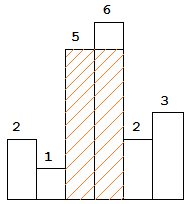
\includegraphics[width = 0.4\columnwidth]{fig/histogram.png}
    \caption{Histogram}
    \label{fig:histogram}
\end{figure}
Above is a histogram where width of each bar is 1, given height = $[2,1,5,6,2,3]$. The largest rectangle is shown in the shaded area, which has area = 10 unit.

Solution: brute force. Start from $2$ which will be included, then we go to the right side to find the minimum height, we could have possible area $(1\times 2, 1\times 3, 1\times 4, 1\times 5, ...)$, which gave us $O(n^2)$ to track the min height and width.
\begin{lstlisting}[language = Python]
class Solution:
    def largestRectangleArea(self, heights):
        """
        :type heights: List[int]
        :rtype: int
        """
        if not heights:
            return 0
        maxsize = max(heights)
        
        for i in range(len(heights)):
            minheight = heights[i]
            width = 1
            for j in range(i+1, len(heights)):
                width+=1
                minheight = min(minheight, heights[j])
                maxsize = max(maxsize,minheight*width)
        return maxsize
\end{lstlisting}
Now, try the BCR, which is $O(n)$. The maximum area is amony areas that use each height as the rectangle  height multiplied by the width that works. For the above example,we would choose the maximum among $2\times 1, 1\times 6, 5\times 2, 6\times 1, 2\times 4, 3\times 1$. So, the important step here is to find the possible width, for element $2$, if the following height is increasing, then the width grows, however, since the following height $1$ is smaller, so $2$ will be popped out, we can get $2\times 1$, which satisfies the condition of the monotonic increasing stack, when one element is popped out, which means we found the next element that is smaller than the kicked out element, so the width span ended here. How to deal if current number equals to previous, 6,6,6,6,6, we need to pop previous, and append current. The structure we use here is called Monotonic Stack, which will only allow the increasing elements to get in the stack, and once smaller or equal ones get in, it kicks out the previous smaller elements.
\begin{lstlisting}[language = Python]
def largestRectangleArea(self, heights):
        """
        :type heights: List[int]
        :rtype: int
        """
        if not heights:
            return 0
        maxsize = max(heights)
        
        stack = [-1]
        
        #the stack will only grow
        for i, h in enumerate(heights):
            if stack[-1]!=-1:
                if h>heights[stack[-1]]:
                    stack.append(i)
                else:
                    #start to kick to pop and compute the area
                    while stack[-1]!=-1 and h<=heights[stack[-1]]: #same or equal needs to be pop out
                        idx = stack.pop()
                        v = heights[idx]
                        maxsize=max(maxsize, (i-stack[-1]-1)*v)
                    stack.append(i)
                
            else:
                stack.append(i)
        #handle the left stack
        while stack[-1]!=-1:
            idx = stack.pop()
            v = heights[idx]
            maxsize=max(maxsize, (len(heights)-stack[-1]-1)*v)
        return maxsize
\end{lstlisting}
85. Maximal Rectangle
Solution: 64/66 with LTE
\begin{lstlisting}[language = Python]
def maximalRectangle(self, matrix):
        """
        :type matrix: List[List[str]]
        :rtype: int
        """
        if not matrix:
            return 0
        if len(matrix[0])==0:
            return 0
        row,col = len(matrix),len(matrix[0])
        
        def  check(x,y,w,h):
            #check the last col
            for i in range(x, x+h): #change row
                if matrix[i][y+w-1]=='0':
                    return 0               
            for j in range(y, y+w): #change col
                if matrix[x+h-1][j]=='0':
                    return 0
            return w*h
        maxsize = 0
        for i in range(row):
            for j in range(col): #start point i,j
                if matrix[i][j]=='0':
                    continue
                for h in range(1, row-i+1): #decide the size of the window
                    for w in range(1,col-j+1):
                        rslt = check(i,j,w,h)
                        if rslt==0: #we definitely need to break it. or else we get wrong result
                            break
                        maxsize = max(maxsize, check(i,j,w,h))
        return maxsize
\end{lstlisting}
Now, the same as before, use the sums
\begin{lstlisting}[language = Python]
def maximalRectangle(self, matrix):
        """
        :type matrix: List[List[str]]
        :rtype: int
        """
        if not matrix:
            return 0
        if len(matrix[0])==0:
            return 0
        row,col = len(matrix),len(matrix[0])
        sums = [[0 for _ in range(col+1)] for _ in range(row+1)]
        #no need to initialize row 0 and col 0, because we just need it to be 0
        for i in range(1, row+1):
            for j in range(1, col+1):
                sums[i][j]=sums[i-1][j]+sums[i][j-1]-sums[i-1][j-1]+[0,1][matrix[i-1][j-1]=='1']
        
        def  check(x,y,w,h):
            count = sums[x+h-1][y+w-1]-sums[x+h-1][y-1]-sums[x-1][y+w-1]+sums[x-1][y-1]
            return count if count==w*h else 0

maxsize = 0
        for i in range(row):
            for j in range(col): #start point i,j
                if matrix[i][j]=='0':
                    continue
                for h in range(1, row-i+1): #decide the size of the window
                    for w in range(1,col-j+1):
                        rslt = check(i+1,j+1,w,h)
                        if rslt==0: #we definitely need to break it. or else we get wrong result
                            break
                        maxsize = max(maxsize, rslt)
        return maxsize
\end{lstlisting}
Still can not be AC. So we need another solution. Now use the largest rectangle in histogram.
\begin{lstlisting}[language = Python]
def maximalRectangle(self, matrix):
        """
        :type matrix: List[List[str]]
        :rtype: int
        """
        if not matrix:
            return 0
        if len(matrix[0])==0:
            return 0
        def getMaxAreaHist(heights):
            if not heights:
                return 0
            maxsize = max(heights)

stack = [-1]

#the stack will only grow
            for i, h in enumerate(heights):
                if stack[-1]!=-1:
                    if h>heights[stack[-1]]:
                        stack.append(i)
                    else:
                        #start to kick to pop and compute the area
                        while stack[-1]!=-1 and h<=heights[stack[-1]]: #same or equal needs to be pop out
                            idx = stack.pop()
                            v = heights[idx]
                            maxsize=max(maxsize, (i-stack[-1]-1)*v)
                        stack.append(i)

else:
                    stack.append(i)
            #handle the left stack
            while stack[-1]!=-1:
                idx = stack.pop()
                v = heights[idx]
                maxsize=max(maxsize, (len(heights)-stack[-1]-1)*v)
            return maxsize
        row,col = len(matrix),len(matrix[0])
        heights =[0]*col #save the maximum heights till here
        maxsize = 0
        for r in range(row):
            for c in range(col):
                if matrix[r][c]=='1':
                    heights[c]+=1
                else:
                    heights[c]=0
            #print(heights)
            maxsize = max(maxsize, getMaxAreaHist(heights))
        return maxsize
\end{lstlisting}

\textbf{Monotonic Stack}

122. Best Time to Buy and Sell Stock II

Say you have an array for which the ith element is the price of a given stock on day i.

Design an algorithm to find the maximum profit. You may complete as many transactions as you like (i.e., buy one and sell one share of the stock multiple times).

Note: You may not engage in multiple transactions at the same time (i.e., you must sell the stock before you buy again).

Example 1:
\begin{lstlisting}
Input: [7,1,5,3,6,4]
Output: 7
Explanation: Buy on day 2 (price = 1) and sell on day 3 (price = 5), profit = 5-1 = 4.
             Then buy on day 4 (price = 3) and sell on day 5 (price = 6), profit = 6-3 = 3.
\end{lstlisting}
Example 2:
\begin{lstlisting}
Input: [1,2,3,4,5]
Output: 4
Explanation: Buy on day 1 (price = 1) and sell on day 5 (price = 5), profit = 5-1 = 4.
             Note that you cannot buy on day 1, buy on day 2 and sell them later, as you are
             engaging multiple transactions at the same time. You must sell before buying again.
\end{lstlisting}
Example 3:
\begin{lstlisting}
Input: [7,6,4,3,1]
Output: 0
Explanation: In this case, no transaction is done, i.e. max profit = 0.
\end{lstlisting}
Solution: the difference compared with the first problem is that we can have multiple transaction, so whenever we can make profit we can have an transaction. We can notice that if we have [1,2,3,5], we only need one transaction to buy at 1 and sell at 5, which makes profit 4.  This problem can be resolved with decreasing monotonic stack.  whenever the stack is increasing, we kick out that number, which is the smallest number so far before i and this is the transaction that make the biggest profit = current price - previous element. Or else, we keep push smaller price inside the stack. 
\begin{lstlisting}[language = Python]
def maxProfit(self, prices):
    """
    :type prices: List[int]
    :rtype: int
    """
    mono_stack = []
    profit = 0
    for p in prices:
        if not mono_stack:
            mono_stack.append(p)
        else:
            if p<mono_stack[-1]:
                mono_stack.append(p)
            else:
                #kick out till it is decreasing
                if mono_stack and mono_stack[-1]<p:
                    price = mono_stack.pop()
                    profit += p-price

                while mono_stack and mono_stack[-1]<p:
                    price = mono_stack.pop()
                mono_stack.append(p)
    return profit
\end{lstlisting}
Also, there are other solutions that can use $O(1)$ space.  Say the given array is: [7, 1, 5, 3, 6, 4]. If we plot the numbers of the given array on a graph, we get:
\begin{figure}[h]
    \centering
    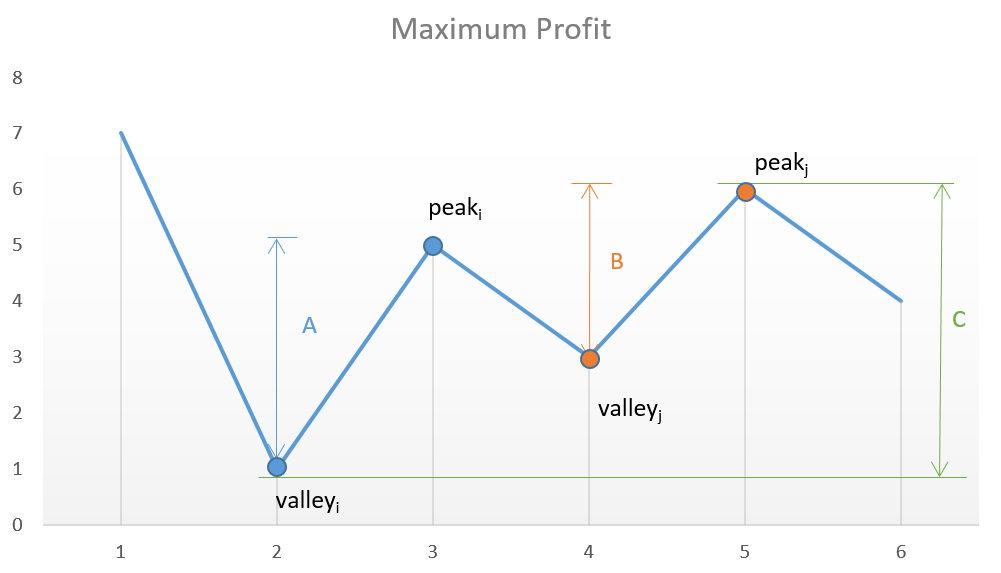
\includegraphics[width = 0.9\columnwidth]{fig/maxprofit_peak.png}
    \caption{Track the peaks and valleys}
    \label{fig:max_profit_peak_valley}
\end{figure}
If we analyze the graph, we notice that the points of interest are the consecutive valleys and peaks.

Mathematically speaking:
\begin{equation}
Total Profit= \sum_{i}(height(peak_i)-height(valley_i)) 
\end{equation}

The key point is we need to consider every peak immediately following a valley to maximize the profit. In case we skip one of the peaks (trying to obtain more profit), we will end up losing the profit over one of the transactions leading to an overall lesser profit.

\begin{lstlisting}[language = Python]
class Solution {
    public int maxProfit(int[] prices) {
        int i = 0;
        int valley = prices[0];
        int peak = prices[0];
        int maxprofit = 0;
        while (i < prices.length - 1) {
            while (i < prices.length - 1 && prices[i] >= prices[i + 1])
                i++;
            valley = prices[i];
            while (i < prices.length - 1 && prices[i] <= prices[i + 1])
                i++;
            peak = prices[i];
            maxprofit += peak - valley;
        }
        return maxprofit;
    }
}
\end{lstlisting}
This solution follows the logic used in Approach 2 itself, but with only a slight variation. In this case, instead of looking for every peak following a valley, we can simply go on crawling over the slope and keep on adding the profit obtained from every consecutive transaction. In the end,we will be using the peaks and valleys effectively, but we need not track the costs corresponding to the peaks and valleys along with the maximum profit, but we can directly keep on adding the difference between the consecutive numbers of the array if the second number is larger than the first one, and at the total sum we obtain will be the maximum profit. This approach will simplify the solution. This can be made clearer by taking this example: [1, 7, 2, 3, 6, 7, 6, 7]

The graph corresponding to this array is:
\begin{figure}[h]
    \centering
    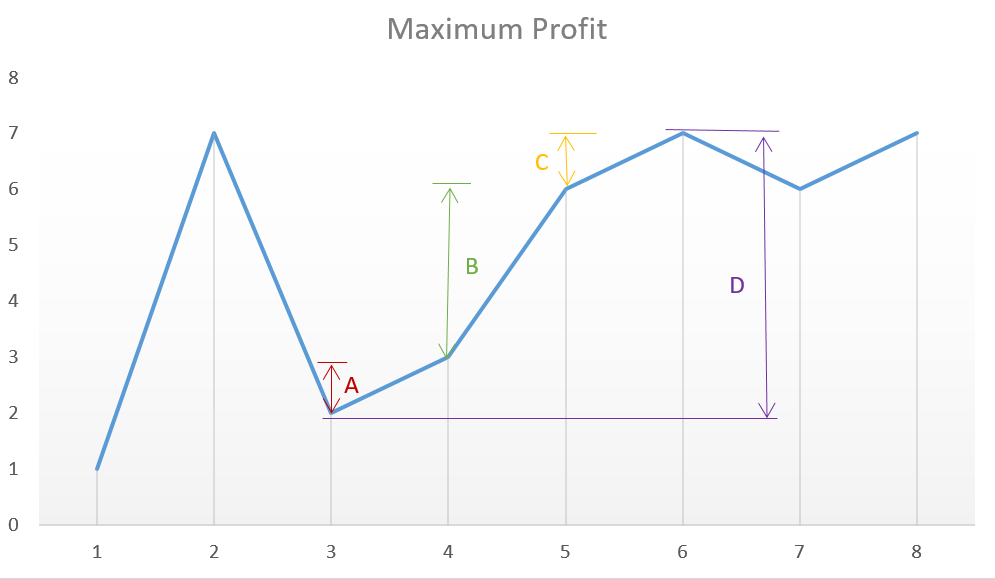
\includegraphics[width = 0.9\columnwidth]{fig/maxprofit_consecutive.png}
    \caption{profit graph}
    \label{fig:profit_graph}
\end{figure}

From the above graph, we can observe that the sum A+B+CA+B+CA+B+C is equal to the difference D corresponding to the difference between the heights of the consecutive peak and valley.
\begin{lstlisting}[language = Python]
class Solution {
    public int maxProfit(int[] prices) {
        int maxprofit = 0;
        for (int i = 1; i < prices.length; i++) {
            if (prices[i] > prices[i - 1])
                maxprofit += prices[i] - prices[i - 1];
        }
        return maxprofit;
    }
}
\end{lstlisting}
\end{examples}
%%%%%%%%%%%%%queue and stack%%%%%%%%%%%%%%%%%%%%%%%
\section{Heap and Priority Queue}
\begin{examples}[resume]
\item \textbf{621. Task Scheduler (medium).} Given a char array representing tasks CPU need to do. It contains capital letters A to Z where different letters represent different tasks. Tasks could be done without original order. Each task could be done in one interval. For each interval, CPU could finish one task or just be idle.

However, there is a non-negative cooling interval n that means between two \textbf{same tasks}, there must be at least n intervals that CPU are doing different tasks or just be idle. You need to return the \textbf{least} number of intervals the CPU will take to finish all the given tasks.
\begin{lstlisting}[numbers=none]
Example:

Input: tasks = ["A","A","A","B","B","B"], n = 2
Output: 8
Explanation: A -> B -> idle -> A -> B -> idle -> A -> B.
\end{lstlisting}

Analysis: we can approach the problem by thinking when we can get the least idle times? Whenever we put the same task together, they incurs largest idle time. Therefore, rule number 1: put different task next to each other whenever it is possible. However, consider the case: {"A":6, "B":1, "C":1, "D":1", "E":1}, if we simply do a round of using all of the available tasks in the decreasing order of their frequency, we get 'A, B, C, D, E, A , ?, A, ?, A, ?, A, ?', here we end up with four '?', which represents idle. However, this is not the best solution. A better way that this is to use up the most frequent task as soon as its cooling time is finished. The new order is 'A, B, C, A, D, E, A, ?, A, ?, A, ?, A'. We end up with one less idle session. We can implement it with heapq due to the fast that it is more efficient compared with PriorityQueue(). 

\textbf{Solution 1: heapq and idle cycle. } We can use a map to get the frequency of each task, then we put their frequencies into a heapq, by using heapify function. When the list is not empty yet, for each idle cycle: which is n+1, we pop out items out and decrease its frequency and add time. (Actually, using PriorityQueue() here we will receive LTE.) We need $O(n)$ to iterate through the tasks list to get its frequency. Then heapify takes $O(26)$, each time, heappush takes $O(\log 26)$. This still makes the time complexity $O(n)$. 
\begin{lstlisting}[language=Python]
from collections import Counter
from queue import PriorityQueue
import heapq
def leastInterval(self, tasks, n):
    c = Counter(tasks)
    h = [-count for _, count in c.items()]
    heapq.heapify(h)

    ans = 0
        
    while h:
        temp = []
        i = 0
        while i <= n: # a cycle is n+1

            if h:
                c = heapq.heappop(h)
                if c < -1:
                    temp.append(c+1)
            ans += 1
            # if the queue is empty, we reached the end, need to break, no idle
            if not h and not temp:
                break
            i += 1
        for c in temp:
            heapq.heappush(h, c)
    return ans
\end{lstlisting}

\begin{figure}[h!]
    \centering
    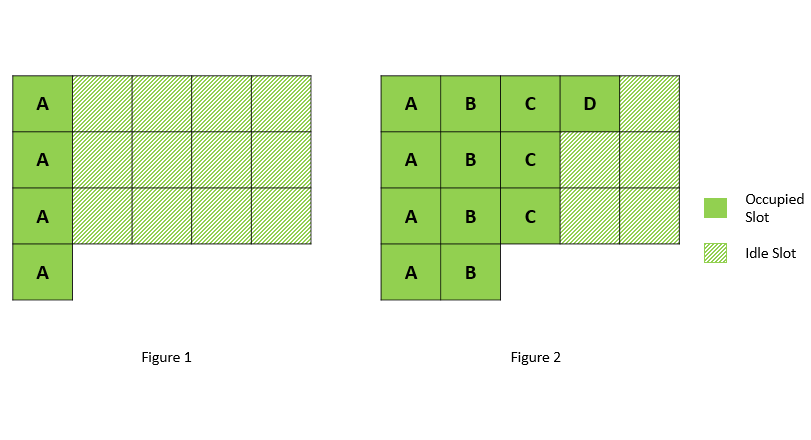
\includegraphics[width = 0.9\columnwidth]{fig/621_Task_Scheduler_new.png}
    \caption{Task Scheduler, Left is the first step, the right is the one we end up with.}
    \label{fig:task_scheduler}
\end{figure}
\textbf{Solution 2: Use Sorting}. Obversing Fig.~\ref{fig:task_scheduler}, the actually time = idle time + total number of tasks. So, all we need to do is getting the idle time. And we start with the initial idle time which is (biggest frequency - 1)*(n). Then we travese the sorted list from the second item, and decrase the initial idle time. This gives us $O(n)$ time too. But the concept and coding is easier. 
\begin{lstlisting}[language=Python]
from collections import Counter
def leastInterval(self, tasks, n):
    c = Counter(tasks)
    f = [count for _, count in c.items()]
    f.sort(reverse =True)
    idle_time = (f[0] - 1) * n
    
    for i in range(1, len(f)):
        c = f[i]
        idle_time -= min(c, f[0]-1)
    return idle_time + len(tasks) if idle_time > 0 else len(tasks)
\end{lstlisting}
\end{examples}
\end{document}